\section{Pianificazione}

La pianificazione del progetto viene suddivisa nelle seguenti fasi:
\begin{itemize}
	\item \textbf{Analisi;}
	\item \textbf{Presentazione;}
	\item \textbf{Progettazione architetturale;}
	\item \textbf{Progettazione di dettaglio e codifica;}
	\item \textbf{Validazione e collaudo;}
\end{itemize}
Ogni fase ha la sua corrispettiva scadenza (vedi 1.5) e viene suddivisa in sotto-attività prima di iniziare la sua implementazione.
\subsection{Analisi}
Questa fase è stata suddivisa nelle attività:
\begin{itemize}
	\item \textbf{Individuazione degli strumenti:} questa attività consiste nel determinare quali strumenti il gruppo deve utilizzare per la comunicazione, per la stesura dei documenti e per il versionamento, lo sviluppo e la verifica del software;
	\item \textbf{Norme di Progetto:} sono definite tutte le regole utili per lo svolgimento del progetto, relative al prodotto da realizzare e ai processi da adottare. Il documento \textit{Norme di Progetto} viene redatto dall’Amministratore per conto del Responsabile di progetto;
	\item \textbf{Studio di fattibilità:} in questa attività gli analisti effettuano uno studio sommario dei capitolati in modo da determinare quale di essi verrà scelto. Questa attività è da considerarsi bloccante per l’attività di Analisi dei Requisiti;
	\item \textbf{Analisi dei Requisiti:} durante questa attività vengono identificati ed analizzati i requisiti del capitolato scelto nell’attività di studio di fattibilità e il relativo documento viene composto dagli Analisti;
	\item \textbf{Piano di Qualifica:} in questa attività si individuano le metodologie attraverso le quali si garantisce la qualità del prodotto. A supporto di ciò viene redatto il documento Piano di Qualifica da parte dell’Amministratore e per la parte programmatica dal Progettista;
	\item \textbf{Glossario:} tutti i termini che possono risultare ambigui vengono individuati e definiti nel documento Glossario, che viene redatto durante tutta la fase di analisi dei requisiti;
\end{itemize}
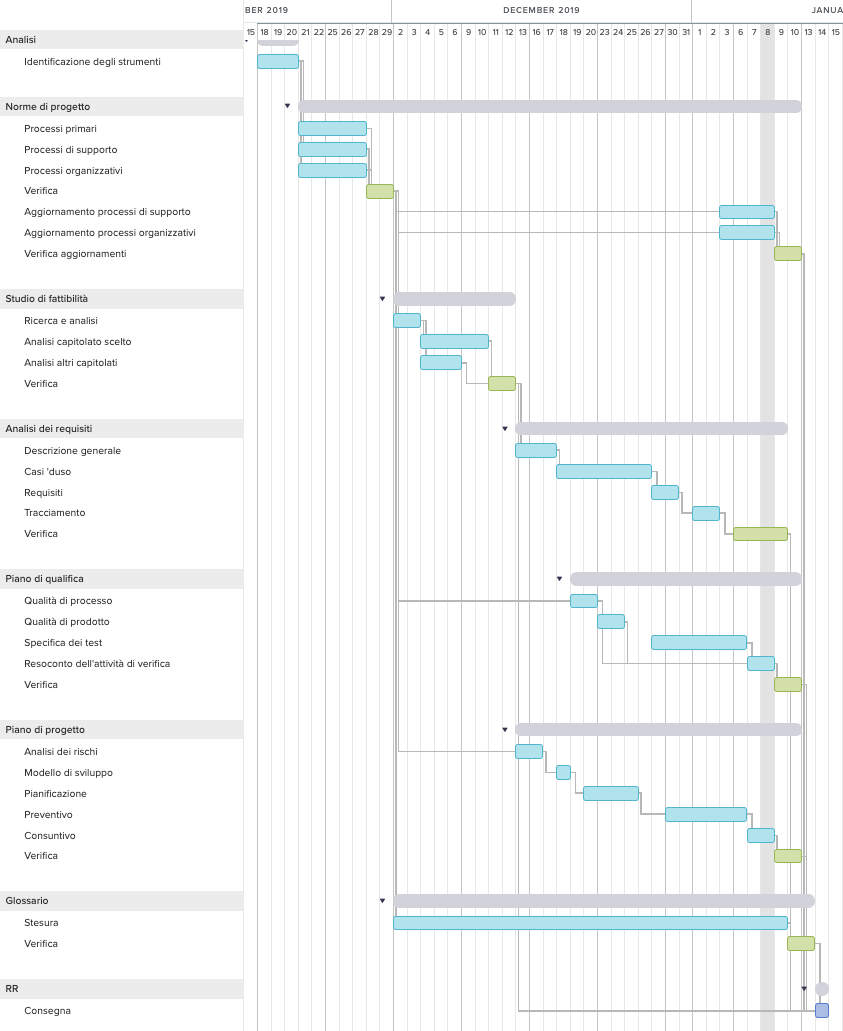
\includegraphics[width=\textwidth]{res/img/g1113}

\subsection{Presentazione}
Questa fase consiste nella realizzazione di una presentazione ed è stata suddivisa nelle attività:
\begin{itemize}
	\item \textbf{Presentazione:} predisposizione e preparazione dei contenuti per la presentazione;
\end{itemize}
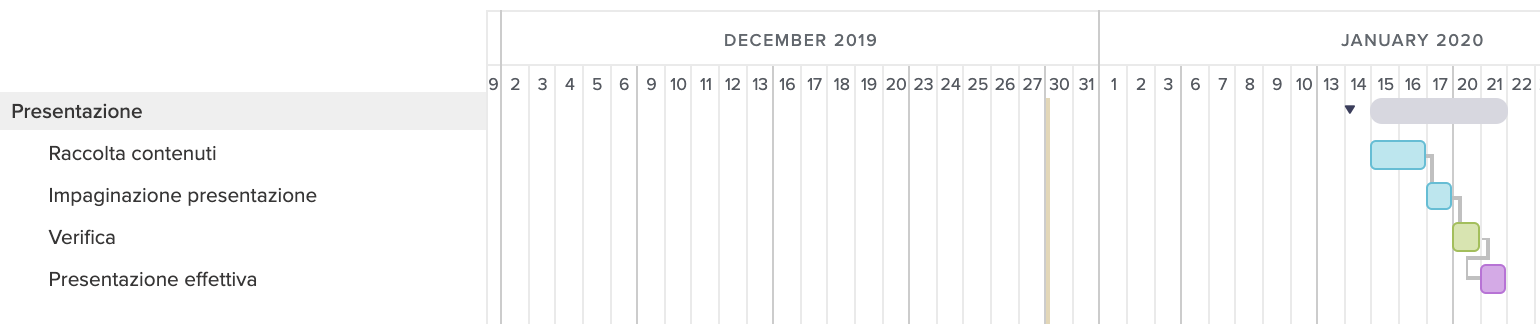
\includegraphics[width=\textwidth]{res/img/g2}

\subsection{Progettazione architetturale}
Questa fase consiste nella individualizzazione di una soluzione architetturale che soddisfi i requisiti del prodotto ed è stata suddivisa nelle sotto-attività:
\begin{itemize}
	\item \textbf{Technology Baseline:} redazione di un documento nel quale vengono individuati e specificati i pattern di programmazione utilizzati negli ambiti delle tecnologie coinvolte;
	\item  \textbf{Proof of concept:} le decisioni prese in questa fase vengono impiegate per la codifica di una bozza del prodotto per verificare la corretta disposizione architetturale dei componenti;
	\item \textbf{Documentazione:} incremento della documentazione in base ai nuovi dati rilevati;
\end{itemize}
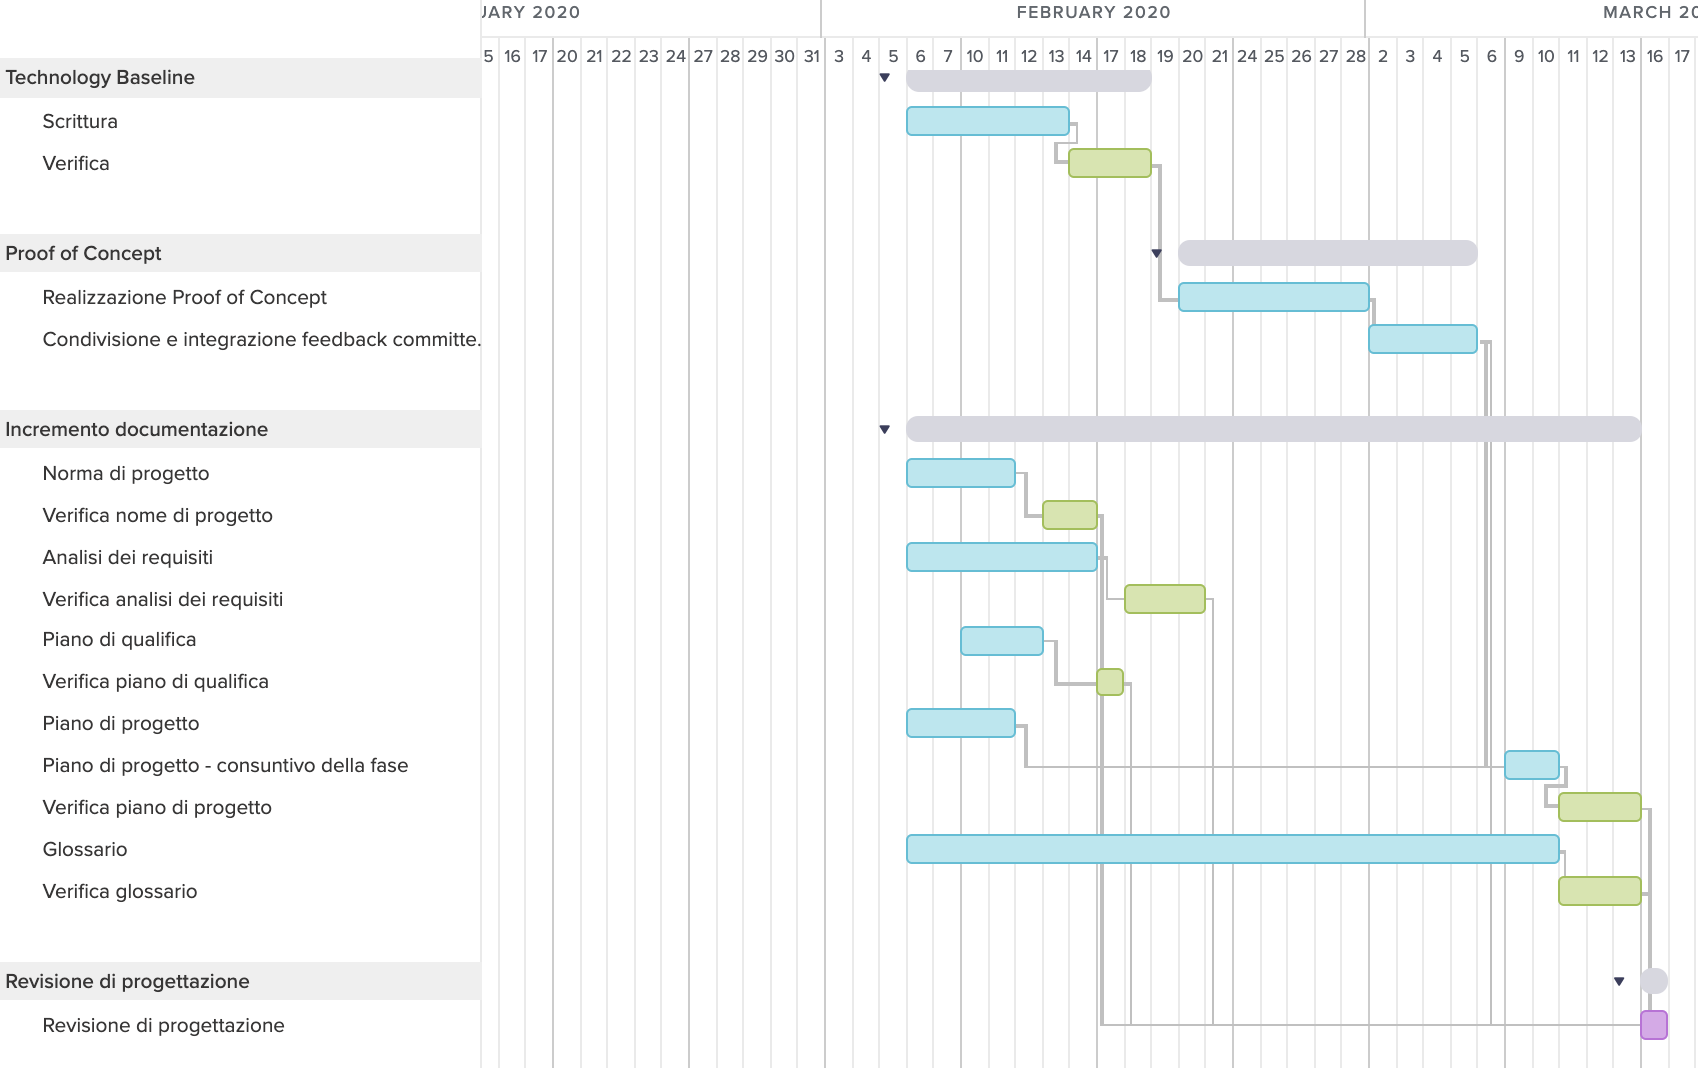
\includegraphics[width=\textwidth]{res/img/g3}

\subsection{Progettazione di dettaglio e codifica}
Questa fase è stata suddivisa nelle attività:
\begin{itemize}
	\item \textbf{Specifiche di prodotto:} redazione di un documento nel quale vengono individuati le componenti atomiche che costituiscono il prodotto; viene fatta una analisi e progettazione approfondita in modo tale da permettere la corretta codifica delle funzionalità;
	\item  \textbf{Codifica:} realizzazione effettiva del prodotto;
	\item \textbf{Manuale utente:} realizzazione del \textit{Manuale Utente} per l'utilizzo del prodotto;
	\item \textbf{Documentazione:} incremento della documentazione in base ai nuovi dati rilevati;
\end{itemize}

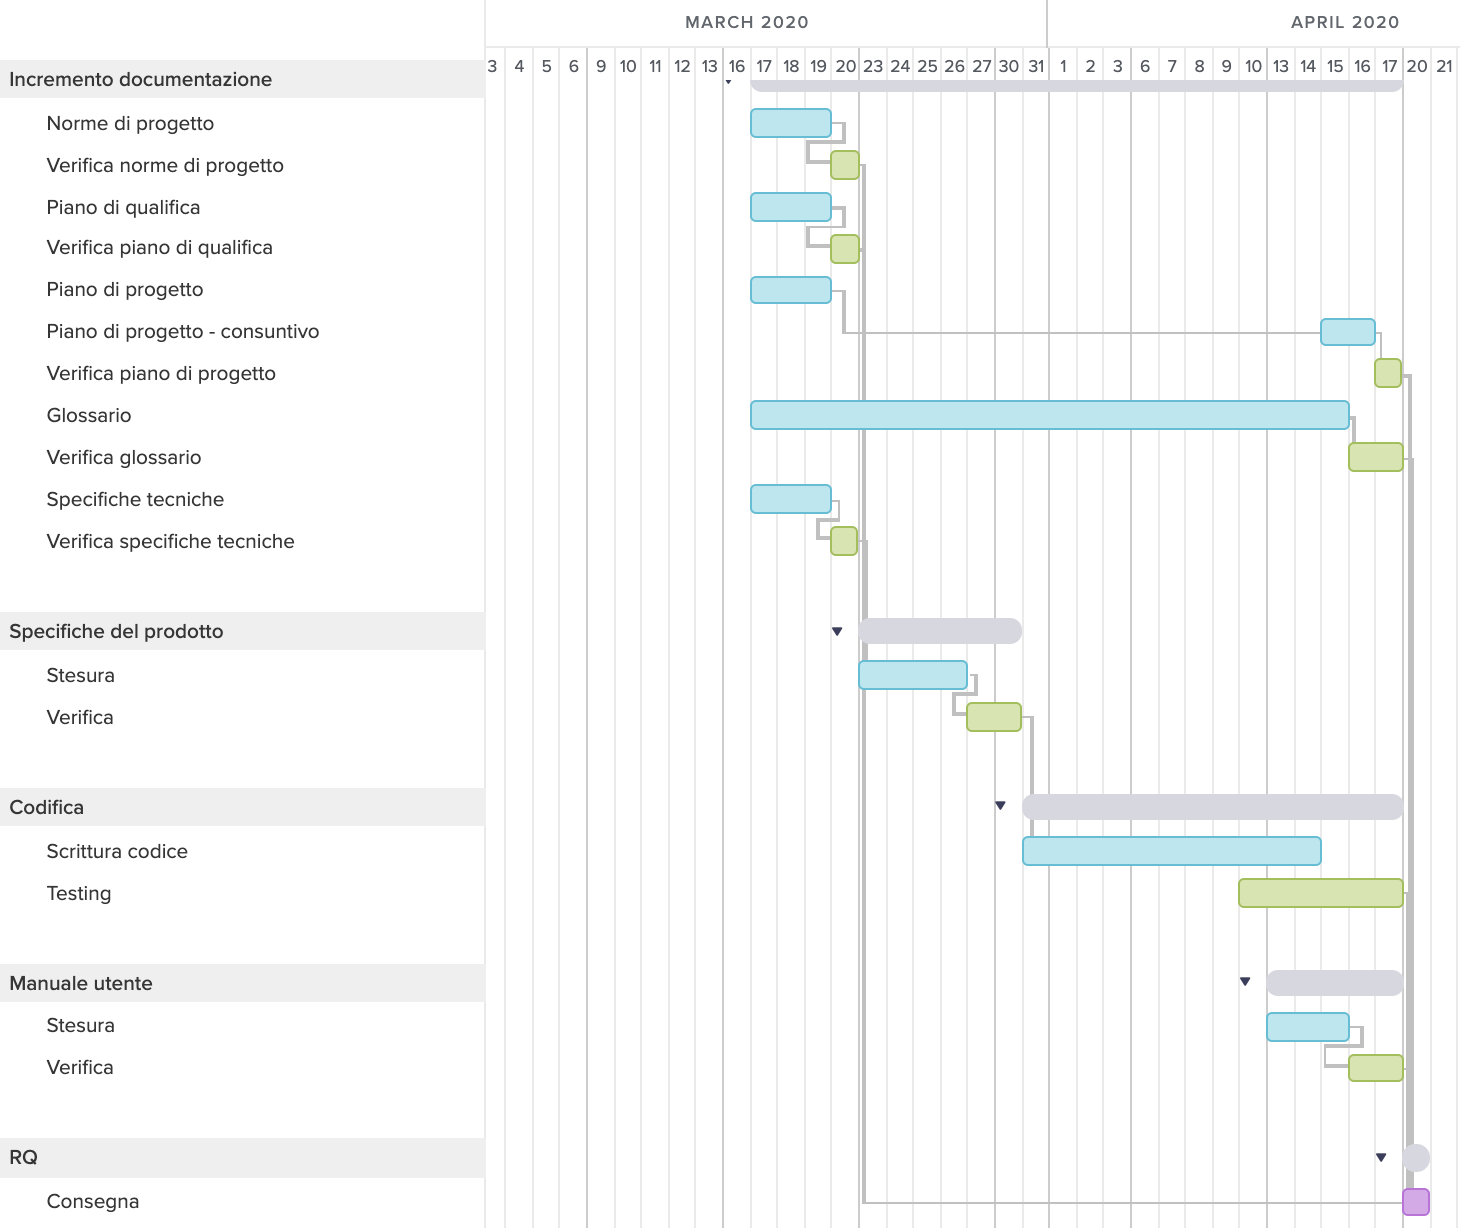
\includegraphics[width=\textwidth]{res/img/g4}

\subsection{Validazione e collaudo}
Questa fase è stata suddivisa nelle attività:
\begin{itemize}
	\item \textbf{Documentazione codice:} realizzazione documentazione relative al codice scritto atto a fornire le conoscenze necessarie per la manutenzione e modifica del programma;
	\item \textbf{Validazione e Collaudo:} controlli per verificare se il prodotto finale è congrue a quanto richiesto nelle specifiche del committente e verifica del corretto funzionamento;
	\item \textbf{Documentazione:} incremento della documentazione in base ai nuovi dati rilevati;
\end{itemize}
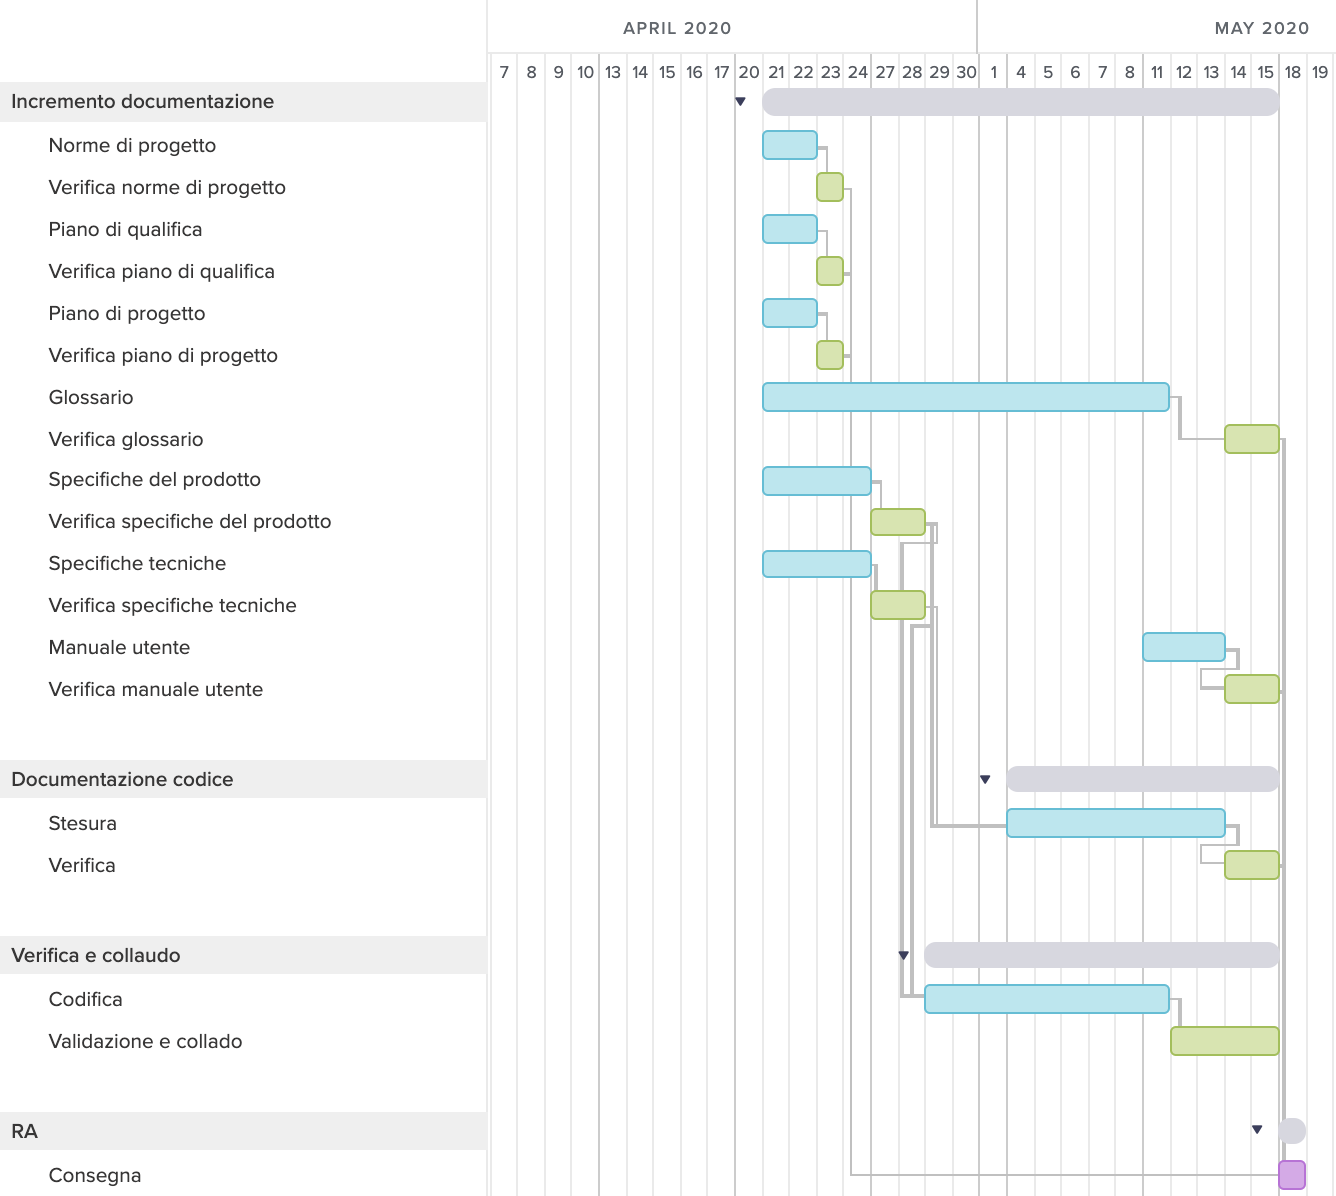
\includegraphics[width=\textwidth]{res/img/g5}